\documentclass[a4paper]{article}

\usepackage[english]{babel}
\usepackage[utf8x]{inputenc}
\usepackage{amsmath}
\usepackage{amssymb}
\usepackage{graphicx}
\usepackage[colorinlistoftodos]{todonotes}

\title{Spectrally grown graphs}
\author{Mats-Erik Pistol\\ Solid State Physics and NanoLund\\ Box 118, Lund University, Lund SWEDEN}

\begin{document}
\maketitle

\begin{abstract}
Quantum graphs have attracted attention from mathematicians for quite some time. A quantum graph is defined by having a Laplacian on each edge of a metric graph and imposing boundary conditions at the vertices to get an eigenvalue problem. Most often Neumann boundary conditions are used. It is fairly straightforward to find the eigenvalues of a graph, but the inverse problem of finding a graph with prescribed eigenvalues is much harder. We approach this inverse problem by "spectrally grown graphs". These are graphs that are evolved from a starting (parent) graph such that their eigenvalues are close to a predefined criterion. This could be to have a spectrum (where only small eigenvalues are considered) which is close to a predefined target spectrum. To evolve the graphs we allow a parent graph to have a set of child graphs. Child graphs are obtained by modifying the parent graph by either adding or deleting an edge. The child graph that has the spectrum that is closest to the predefined spectrum is allowed to survive and get child graphs on its own. Our experiments reveal that the selection criteria (goals) strongly influence the shape of the evolved graphs. We have also developed a way to program the evolution of the graphs where different goals are set in succession.
We hope that our software will be useful for mathematicians studying quantum graphs. We have found that experimenting with the spectral growth of graphs makes it easy to find new conjectures and one such is given.

\end{abstract}

\section{Introduction}

Quantum graphs have been studied for several decades. A quantum graph \cite{kuchment2004quantum} is a metric graph, $\Gamma$, such that 
with each edge we have associated an ordinary differential equation. Introducing in addition matching conditions at the vertices make the operator self-adjoint.
In the current paper we reduce our analysis to the simplest case of Laplace differential operator defined on functions satisfying so-called standard vertex conditions (see (\ref{sc}) below).
Then the spectrum of the operator is often refereed to as the spectrum of the graph $ \Gamma. $ It is important to 
remember that  there are graphs that are not isomorphic but still have the same spectrum \cite{gutkin2001can}. 
There is a wide literature describing the relations between the topological and metric properties of a finite graph $ \Gamma $ and its spectrum \cite{kennedy2015spectral, berkolaiko2013introduction}.
For example the spectrum determines the total length of the metric graph and its Euler characteristic \cite{KurArkiv,KurJFA}.

  It is not particularly easy to obtain the eigenvalues of a graph which hampers progress. This is the problem that we were able to solve to some extent by creating a computer  program that gives the eigenvalues of a finite graph. For simple graphs we get \emph{all} eigenvalues analytically. In fact, we do get analytical solutions for surprisingly difficult graphs.
 
 Having such a program allows us not only to study spectra of sophisticated graphs and guess estimates on the eigenvalues.
 One of the main contributions of our paper is formulation of a new type of evolution that 
 we call {\bf spectrum driven dynamics}. The spectrum (in our case the eigenvalues) provide an important global characteristic of the system. Therefore it appears natural to define
 a certain evolution using just the eigenvalues. Such evolution reminds  Loewner evolution, where the dynamics (determined by Loewner's equation)
 is defined in terms of the function giving the conformal map. Such map (as the spectrum in our case) provides a global characteristic of the curve which is changing.
 We consider the simplest discrete case of spectrum driven dynamics for quantum graphs, where the new graph is obtained by adding one new edge to the original
 graph. There are finitely many graphs to choose between. One picks up the graph (which may not be unique) that satisfies certain criteria formulated in terms of its 
 spectrum. For example one may choose the new graph with the smallest spectral gap (the difference between the lowest two eigenvalues). 
 Then it is not surprising that
 one gets in the limit the graph that reminds single  interval, since the interval is the minimiser of the spectral gap among the graphs having the same total length.

The law how to  choose the next graph on each step can be different and should reflect our task.  Our goal is to carry out experiments
illustrating which new features the new evolution may demonstrate. In particular we investigate the following evolution laws:
\begin{itemize}
\item One choses first a certain target spectrum (few first eigenvalues), the new graph is chosen having the spectrum closest to the target.
\item The new graph is chosen minimising one of the eigenvalues, their ration or any other algebraic combination.
\end{itemize}
 
We have found that experimenting with spectral growth of graphs quickly leads to interesting conjectures. One such, concerning the distribution of the first eigenvalues of dumbbell graphs, is given. 



\section{Laplacians on graphs and their spectra}

In this section we briefly define the main object of our studies -- the differential Laplace operator on a metric graph $ \Gamma. $
Consider any finite compact metric graph $ \Gamma $ formed by joining together $ N $ edges $ E_n, \; n=1,2, \dots N $ at $ M $
vertices $ V_m, m=1,2, \dots, M. $ Each edge $ E_n $ is identified with a compact interval $ [x_{2n-1}, x_{2n}] $ on the real line.
Then the (standard) Laplace operator $ L = - \nabla^2 $ is defined on the functions satisfying standard (Kirchhoff, Neumann) vertex conditions:
\begin{equation} \label{sc}
\left\{
\begin{array}{ll}
\displaystyle  f(x_i)=f(x_j), & x_i, x_j \in V_m, \\[3mm]
\displaystyle \sum_{x_{ \in V_m} i}\partial_{n}f(x_i)=0. &
\end{array} \right. 
\end{equation}
at each vertex $ V_m$ where the $x_i$'s are the endpoints of the edges that meet at the vertex. In words, the eigenfunctions are required to be
continuous at the vertex and the sum of their normal derivatives, $\partial_{n}f(x_i)$, at the vertex is zero. The operator so defined
is self-adjoint \cite{berkolaikokuchment,kostrykin1999kirchhoff}. 

 Our main interest is
the spectrum of the standard Laplace operator $ L$.  The spectrum if formed by all $ \lambda = k^2 $ such that the equation $ L \psi = \lambda \psi $
has a non-trivial solution. Every such function $ \psi $ is a solution to the differential equation $ - \psi'' (x) = \lambda \psi $ on every edge
and satisfies vertex conditions at every vertex. The operator $ L $ is nonnegative since its quadratic form is given by
$$ \langle L  u, u \rangle_{L_2(\Gamma)} = \int_\Gamma \vert u' (x) \vert^2 dx \geq 0. $$
The spectrum of the operator is discrete and is formed by a sequence of eigenvalues tending to $ + \infty. $

First of all we note that $ \lambda_0 = 0 $ is an eigenvalue with the eigenfunction $ \psi_0 (x) \equiv 1 $. It is easy to see that this eigenfunction is unique, provided $ \Gamma $ is connected.

Consider now any $ \lambda = k^2 > 0 .$
 The solution of the differential equation on each edge is given by a linear combination of $e^{i k x}$ and $e^{-i k x}$. Imposing the vertex conditions on the eigenfunctions gives a linear equation system which has a solution if a certain $k$-dependent determinant, $D(k)$, is zero. One possible way is to consider these equations as a certain scattering process arriving to the following secular equation
 \begin{equation}
 D(k) := \det \left( S_e (k) S_v - I \right) = 0,
 \end{equation}
 where $ S_e (k) $ is the edge scattering matrix formed by $ 2 \times 2 $ matrices $$ \left(
 \begin{array}{cc}
 0 & e^{ik \ell_n} \\
 e^{ik \ell_n}  & 0
 \end{array} \right) ,$$
 $ \ell_n $ being the length of the corresponding edge $ E_n,$
  and $ S_v $ is the vertex scattering matrix formed by $ d_m \times d_m $ scattering matrices 
 $$ S^m = \left(
 \begin{array}{ccccc}
 -1 + 2/d_m & 2/d_m & 2/d_m & \dots & 2/d_m \\
 2/d_m & -1 + 2/d_m & 2/d_m & \dots & 2/d_m \\
 2/d_m & 2/d_m & -1 + 2/d_m & \dots & 2/d_m \\
 \vdots & \vdots & \vdots & \ddots & \vdots \\
  2/d_m & 2/d_m & 2/d_m & \dots & -1 + 2/d_m \\
 \end{array} \right) ,$$
 with $ d_m $ being the valency of the vertex $ V_m. $
 Observe that the matrices $ S_e $ and $ S_v $ have block-diagonal forms in different bases. For example these marices for the graph depicted in Fig. 1 are as follows:
 $$ S_e (k) =
 \left(
 \begin{array}{cccccccc}
 0 & e^{ikc1} & 0 & 0 & 0 & 0 & 0 & 0 \\
 e^{ikc1} & 0 & 0 & 0 & 0 & 0 & 0 & 0 \\
      0 & 0 & 0 & e^{ik\pi} & 0 & 0 & 0 & 0 \\
  0 & 0 & e^{ik \pi} & 0 & 0 & 0 & 0 & 0 \\
   0 & 0 & 0 & 0 & 0 & e^{ikc1} & 0 & 0 \\
    0 & 0 & 0 & 0 & e^{ikc1} & 0 & 0 & 0 \\
     0 & 0 & 0 & 0 & 0 & 0 & 0 & e^{ikc2} \\
      0 & 0 & 0 & 0 & 0 & 0 & e^{ikc2} & 0 \end{array} \right) ,$$
      $$  S_v = \left(
      \begin{array}{cccccccc}
     -1/3 & 0 & 0 & 0 & 0 & 2/3 & 2/3 & 0 \\
     0 & 0 & 1 & 0 & 0 & 0 & 0 & 0 \\
     0 & 1 & 0 & 0 & 0 & 0 & 0 & 0 \\
     0 & 0 & 0 & 0 & 1 & 0 & 0 & 0 \\
     0 & 0 & 0 & 1 & 0 & 0 & 0 & 0 \\
     2/3 & 0 & 0 & 0 & 0 & -1/3 & 2/3 & 0 \\
     2/3 & 0 & 0 & 0 & 0 & 2/3 & -1/3 & 0 \\
     0 & 0 & 0 & 0 & 0 & 0 & 0 & 1 \\
\end{array} \right) .$$ 
 A description of how to obtain this determinant is given by Gutkin and Smilansky \cite{GS} and in Kurasov and Nowaczyk \cite{kurasov2005inverse} (with an example by Nowaczyk \cite{nowaczyk2005inverse}) and we will not repeat this description here. The most important property of the function $ D(k) $ is that it is an analytic function (trigonometric polynomial) and all its zeroes
 are real having orders equal to the multiplicities of the corresponding eigenvalues, may be with the exception of the eigenvalue $ \lambda_0 = 0. $
 
 In what follows we are going to call the spectrum of the standard Laplace on a metric graph $ \Gamma $ by the spectrum of $ \Gamma.$
  One important observation is that the spectrum scales in an easy way as the lengths of all edges are scaled simultaneously, hence it is natural
  to normalise the graphs so that they have total length equal to one.
 
 
 
 \section{Spectrum driven dynamics}
 
 
 There is a wide literature devoted to different grow models for graphs. Most of these models have probabilistic or random nature. Some models, probably motivated by applications,
 use local rules \cite{vazquez2003growing}. One of the examples here is crystal growth motivated by ice crystals and snow flakes. Our growth process is highly non-local, since 
 the spectra of quantum graphs are very sensitive to the overall graph structure and cannot be determined by a subgraph of the graph.
 Spectrum of a system is one of its most important global characteristic encoding information about its topology and geometry.  
 Our goal is to examine the possibility to determine the evolution itself in terms of the spectrum alone and we are planning to do this using quantum graphs
 as a tool. 
 
 
 Below we describe the most elementary variant of spectrum driven dynamics and discuss its possible generalisations. 
 In order to determine such dynamics, let us choose any {\bf target spectrum} $
  \sigma^* = \{ \mu_0, \mu_1, \mu_2, \dots, \mu_N \} \subset \mathbb R $ with $ \mu_0 = 0 $ and a {\bf length parameter} $ \ell \ll 1 $. 
  The role of the initial condition is played by any finite compact metric graph $ \Gamma_0. $
  
  The evolution is determined using the following inductive procedure
 \begin{enumerate}
 \item {\bf Base} 
 \newline We start from any initial graph $ \Gamma_0 $ and generate a sequence of graphs $ \Gamma_n $ using the
 following
  \item {\bf Induction rule}: 
  \newline Assume that the graph $ \Gamma_n $ is known, then the graph $ \Gamma_{n+1} $
  is constructed following the steps: 
  \begin{itemize}
  \item Calculate the spectrum of $ \Gamma_n $;
  \item Consider all possible graphs obtained by attaching a new edge of length $ \ell \ll 1 $ to one of
  the vertices as a pendant edge or between any  two existing vertices;
    \item Scale the new graphs to meet the normalisation requirement of total length one;
  \item Calculate the spectra of all such graphs and choose the one with the spectrum closest to the target spectrum $
  \sigma = \{ \mu_0, \mu_1, \mu_2, \dots, \mu_N \}. $ Denote one of the optimal graphs by $ \Gamma_{n+1}. $
  \end{itemize}
  \item Repeating the induction procedure one obtains an infinite sequence of metric graphs.
 \end{enumerate}
  The distance between the actual spectrum  $ \sigma (\Gamma_{n}) = \{ \lambda_0,  \lambda_1, \dots \} $ and the target spectrum $ \sigma^* $ is the usual Euclidean distance
  \begin{equation}
  \left( \sum_{n=0}^N \vert \lambda_n- \mu_n \vert^2 \right)^{1/2} . 
  \end{equation}
  
  Our main goal is to study properties of such a sequence and its possible convergence. It is natural to consider the index $ n $ as a certain time-parameter
  and speak about time evolution of the graph. This evolution certainly depends   on the induction rule, but the role of the initial state (graph $ \Gamma_0 $)
  is also important. 
  
  
  
  
  The formulated grow model can be generalised in many ways and it is not our goal to examine all such possibilities:
  \begin{itemize}
  \item the class of allowed graphs may be constrained by, for example, considering only trees;
  \item the notion of the distance between the two spectra can be amended - any distance can be used;
  \item instead of adding one edge, one may add an arbitrary {\it small} graph;
  \item one may allow to delete existing edges or to collapse cycles;
  \item any point on an edge may be considered as a degree two vertex, hence it is natural to allow to add edges between any two points 
  on a metric graph;
  \item instead of having a target spectrum, one may choose another rule like picking up the graph maximising (or minimising) the spectral gap 
  or the entropy. $ $ 
  \end{itemize} 
  
  
  
  
  
  Our focus will be on the topological and geometric properties of the graphs. Since our understanding of these properties is far from being
  satisfactory, search for induction rules that determine interesting evolution requires checking new ideas and  examining different possibilities.
   Our studies show that the dynamics is extremely sensitive to the target spectrum which makes it into a challenging problem to choose the
 target spectrum so that the graphs in the sequence have interesting properties. On the other hand choosing the induction rule in a special way
 one may expect the generated graph sequence will converge to a graph having certain extremal properties. 
  
    
 Introducing spectrum driven dynamics we have two goals:
 \begin{itemize}
 \item Define a deterministic dynamics for metric graphs leading to non-trivial topological models.
 \item Study extremal properties of graph systems.
 \end{itemize}
 



\section*{Graph in Fig 1}

I decided to calculate analytically the spectrum of the graph presented in Fig 1.

We introduce coordinates: $ x= 0 $ in the middle of the left interval, $y= 0$ - the most right end point

The left three intervals can be considered as a loop of length $ 3 \pi$.

Obviously all eigenfunctions can be divided into two classes:

\begin{itemize}

\item symmetric $ = $ invariant under the change of variables: $ x \rightarrow - x, y \rightarrow y. $

\item antisymmetric $ - $ multiplied by $ -1 $ under the change of variables: $ x \rightarrow - x, y \rightarrow y. $
  \end{itemize}

Obviously antisymmetric functions are equal to zero on the right interval.

{\bf Antisymmetric functions}
$$
\psi = \left\{
\begin{array}{cc}
sin kx, &\mbox{on the loop,}\\
0, & \mbox{on the right edge.}
\end{array} \right. $$
The continuity condition at the central vertex gives us:
$$\sin 3 \pi/2 = 0  \Rightarrow k = 2 n/3, n = 1,2, \dots .$$
The condition on the sum of normal derivaties is satisfied automatically.


\section{Program use}





Our program is written in the computer language Mathematica. Graphs are specified in two different ways, either directly by Mathematica commands or by their adjacency matrix. The edge lengths are stored in the elements of the matrix. Two edges can be given symbolic lengths, $c1$ and $c2$. The program normalizes the graphs to length one, where the length is the sum of the length of the edges. The program obtains the eigenvalues, $\lambda=k^2$, using three different methods. In the first method we simply plot the value of $D(k)$ as a function of $k$ and obtain the roots visually. $D(k)$ also contains $c1$ and $c2$ and it is possible to adjust these parameters interactively using sliders and get a feeling for how the roots depend on these parameters. Figure 2 presents $D(k)$ for the graph shown in Figure 1. $c1=\pi$ and $c2$ has been varied from zero to $\pi$ to $50\pi$. Inspecting the graphs we notice a problem. It can happen that $D(k)\leq 0$ in an interval and it is then difficult to know if  $D(k)=0$ within the interval or if it just becomes close to zero, i. e. $D(k) < 0$. This problem can be seen in the left panel in Fig. 2, where $D(k) \leq 0$ for all $k$. A further problem is that even if one knows that $D(k)=0$, due to  $D(k)$ changing sign, it is difficult to know the multiplicity of the root without further investigations.

The program can also compute the zeroes of $D(k)$ numerically and sometimes analytically. Analytical solutions are naturally very hard, and most often impossible, to obtain in many cases. However, surprisingly difficult cases can be solved. For instance the graph in Figure 1 has analytical solutions when $c1=c2=\pi$. The roots are:
\begin{align}
&k=8 \pi n \nonumber \\ 
&k= -(8/3) \pi+ 8 \pi n \nonumber \\
&k=(8/3) \pi+ 8 \pi n \nonumber \\
&k=-4 (\cot^{-1}(x_1) -\pi) + 8 \pi n \\
&k=4 (\cot^{-1}(x_1) -\pi) + 8 \pi n \nonumber \\ 
&k=-4 \cot^{-1}(x_2) + 8 \pi n \nonumber \\
&k=4 \cot^{-1}(x_2) + 8 \pi n \nonumber
\end{align}

Here $x_1$ is the largest and $x_2$ the second largest root of:
\begin{align}
16 x^4 - 19 x^2 + 1=0
\end{align}
and $n\in Z$. Our program manages to find analytical solutions for many other values of $c1$ and $c2$ as well, but not for all.
If we compute the roots numerically we also get all roots in many cases, but certainly not all. Often the calculation has to be aborted due to excessive computing time. There is also an option to find roots in an interval and the graphical output is then useful to determine a suitable interval. In such cases the program tends to find the root. $D(k)$ can be a very complicated function and finding the roots numerically is not trivial.
When we use numerics we can have problems to distinguish between the cases $D(k)\leq 0$ and $D(k) < 0$ on an interval if $D(k)$ does not change sign, due to the finite numerical precision by the software. The numerical precision can be changed but will always be limited.

Despite these shortcomings we have found our program to be very useful to gain understanding of the spectra of different graphs. We often use a combination of plotting $D(k)$ and numerical root finding of $D(k)$. The raison d'\'etre for our program is mostly to introduce experimentation into the field of quantum graphs and possible insights should be proven rigorously.
\begin{figure}
\centering
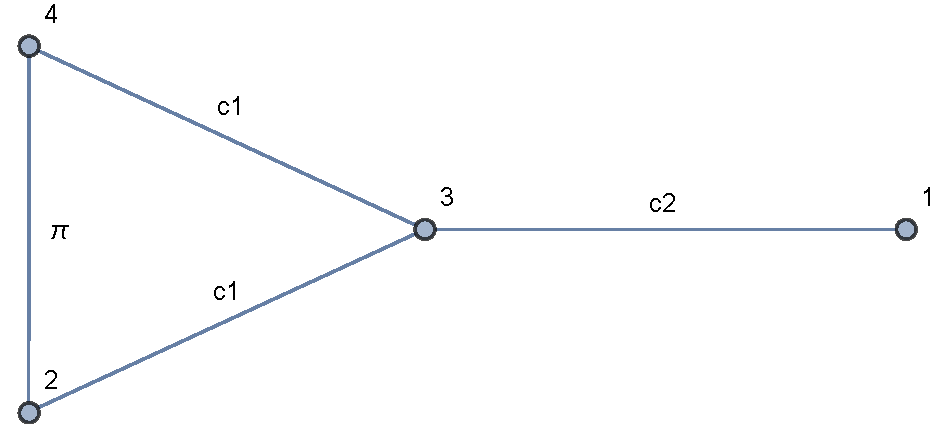
\includegraphics[width=0.7\textwidth]{graph.pdf}
\caption{\label{fig:graph}An example of a metric graph generated by our program. The vertices are labeled by numbers and the edge lengths are indicated. $c1$ and $c2$ are  parameters.}
\end{figure}


\begin{figure}
\centering
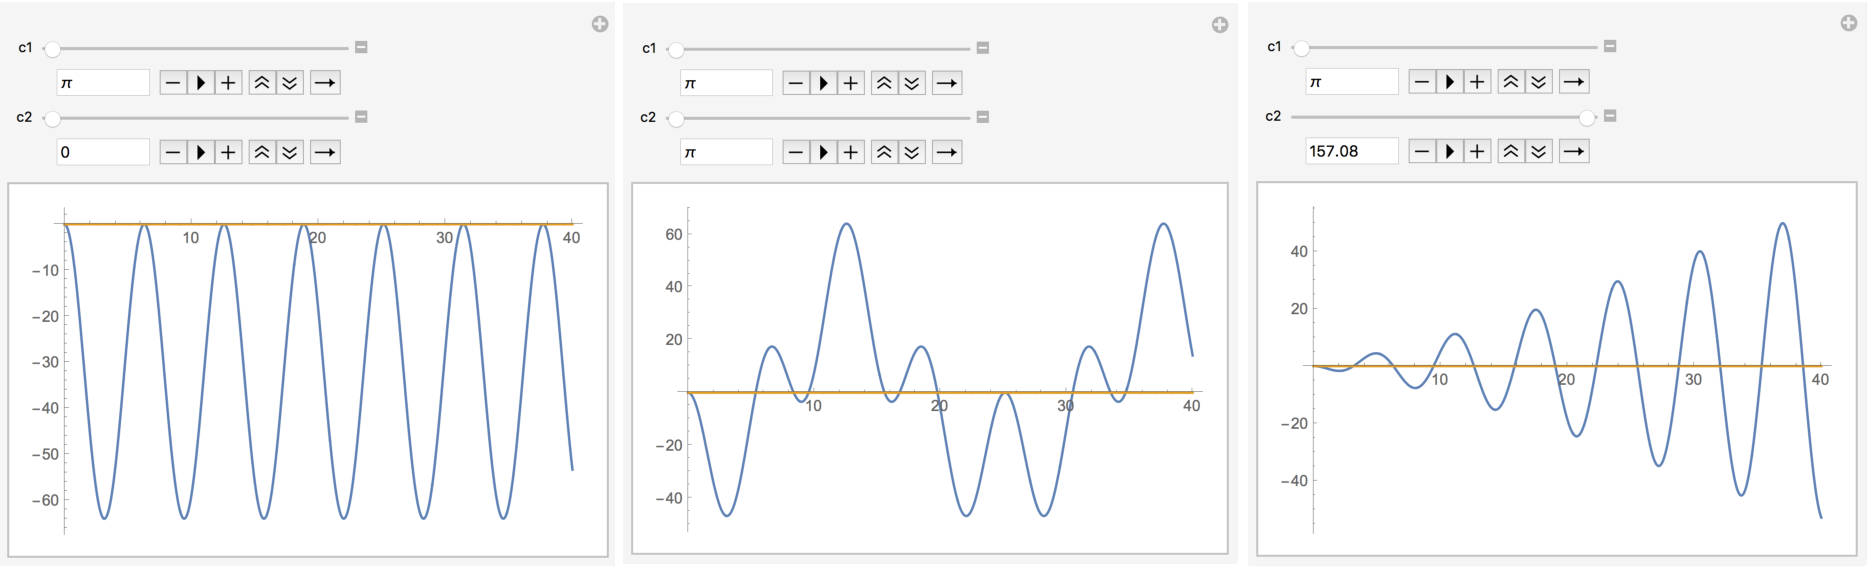
\includegraphics[width=1.0\textwidth]{all.pdf}
\caption{\label{fig:all}Examples of plots of $D(k)$, for the graph shown in Fig. 1, where $c1$ and $c2$ can be changed using sliders. Left panel. Here $c1=\pi$ and $c2=0$ and we have a triangular graph (with length normalized to one). The zeros of $D(k)$ are then at $k=2n\pi$ which is reflected in the figure. Middle panel. Here $c1=c2=\pi$ and it is less obvious where the zeros of $D(k)$ should be located. Right panel. Here $c2=50\pi$ and the graph is almost a path graph, which has zeros of $D(k)$ at $k=n\pi$.}
\end{figure}

\section{Experiments}


\begin{figure}
\centering
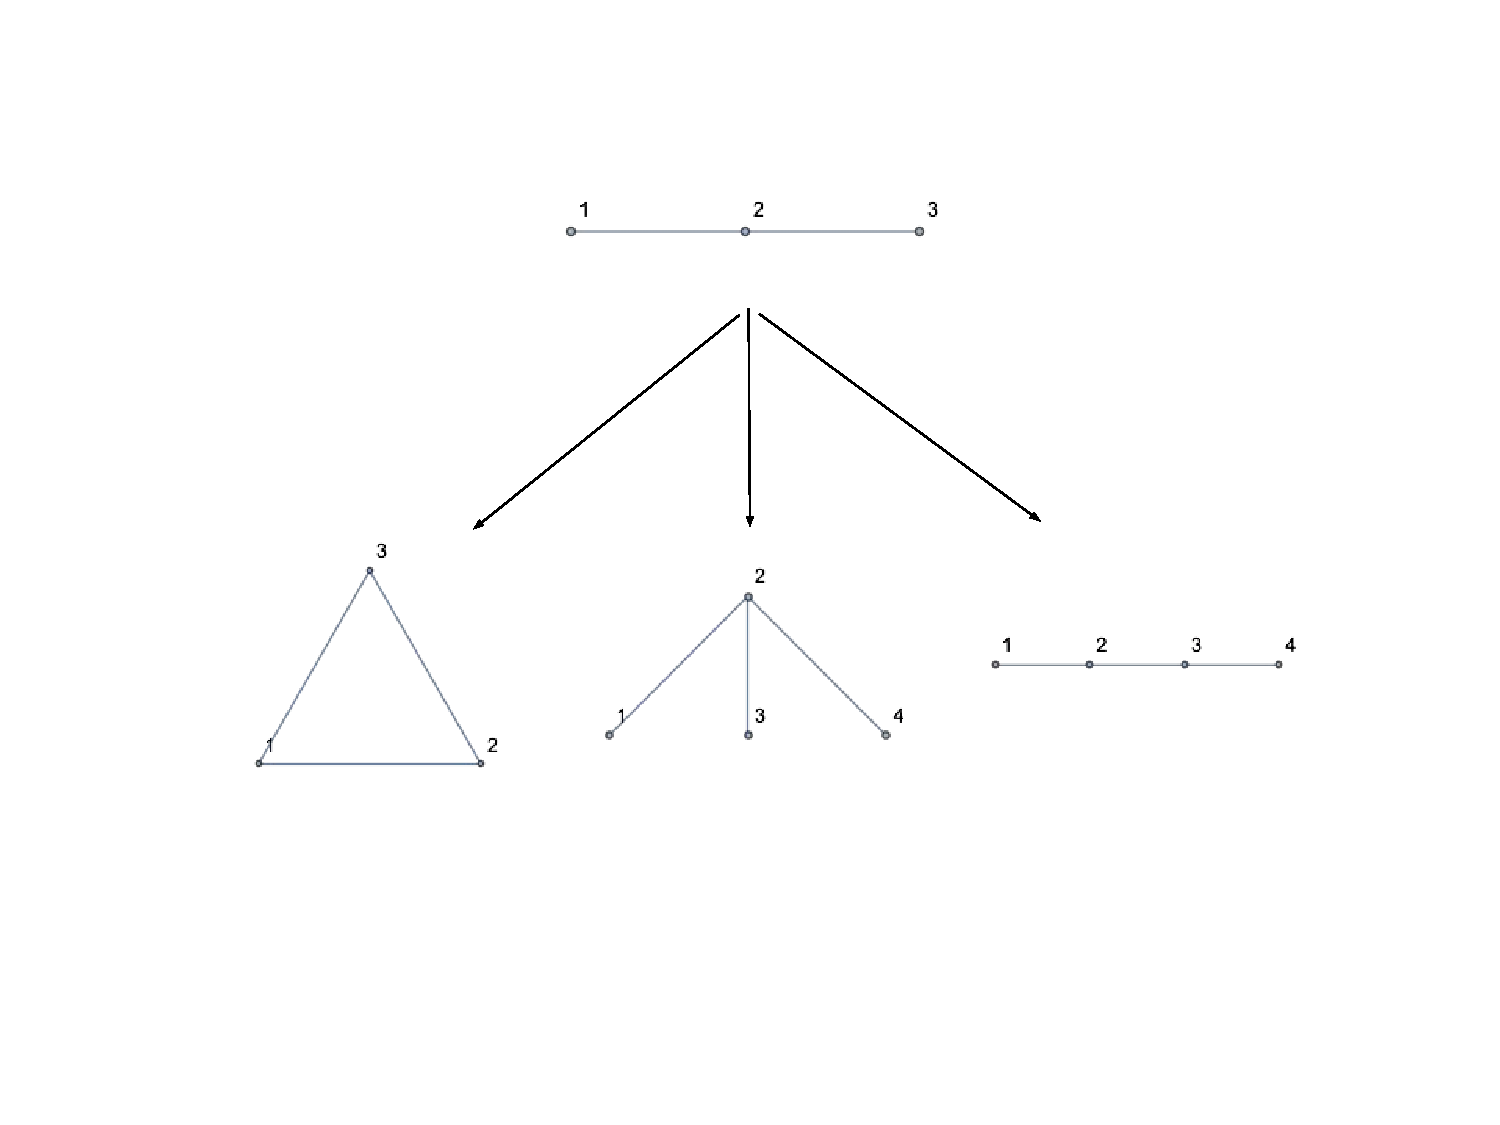
\includegraphics[width=0.5\textwidth]{Parent-child.pdf}
\caption{\label{Parent-child:all}The top graph is the parent graph and has three vertices. From this graph we get three child graphs by adding an edge, shown in the bottom. Out of these child graphs we select the graph which has a spectrum which best fit some chosen criterion. The selected graph becomes a new parent graph and the process is repeated. Note that adding an edge does not necessarily add a vertex.}
\end{figure}





\begin{figure}
\centering
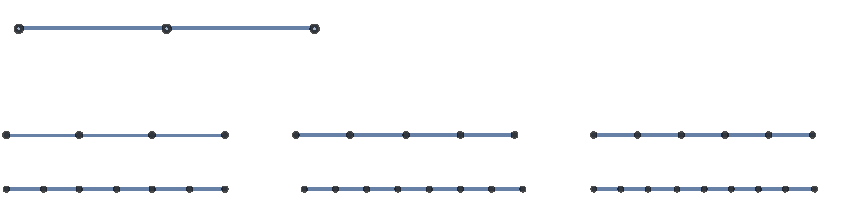
\includegraphics[width=1.0\textwidth]{EdgeGrowth.pdf}
\caption{\label{EdgeGrowth:all}The top graph is the parent graph and has three vertices. From this graph we get the sequence of graphs below. The goal was to have a spectrum with an initial segment which is close to $(0, \pi, 2 \pi)$. This is satisfied by a path graph. The parent graph is simply extended when we evolve the graphs.}
\end{figure}

\begin{figure}
\centering
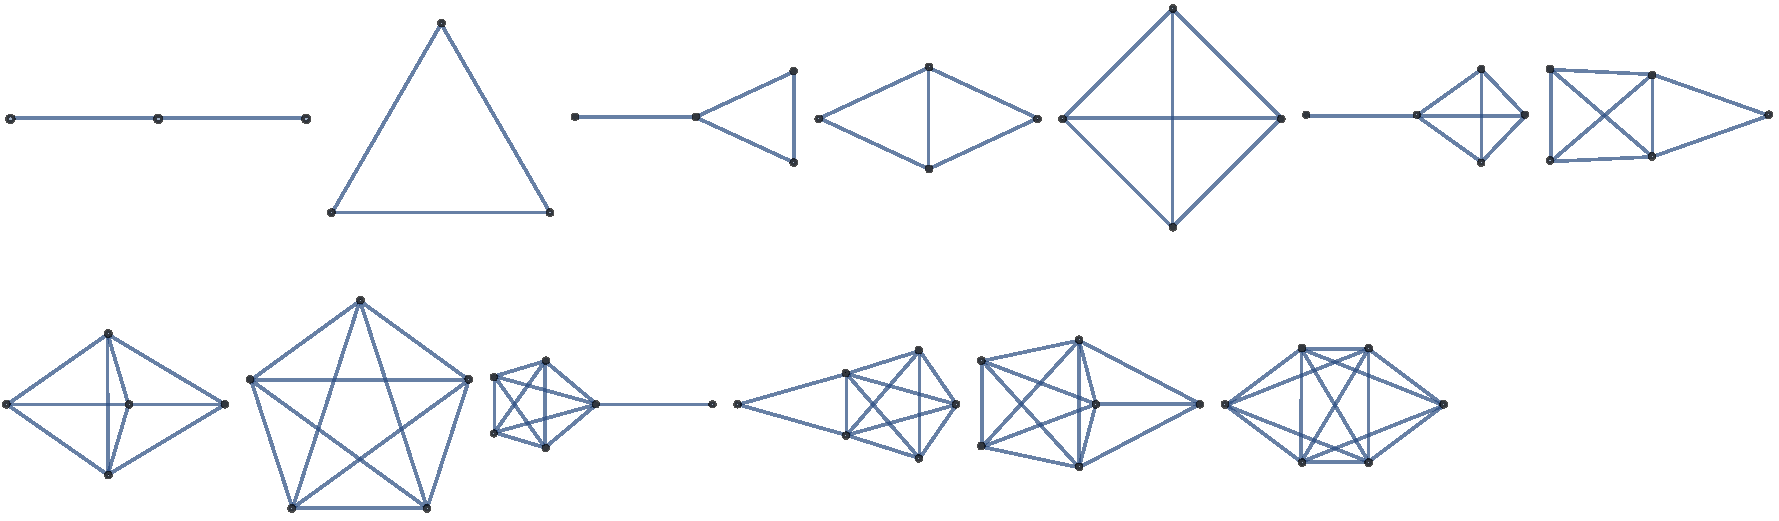
\includegraphics[width=1.0\textwidth]{MaxSpectralGap.pdf}
\caption{\label{MaxSpectralGap:all}In this sequence of graphs the goal was to maximise the spectral gap, $\lambda_{1}$. The graphs are now graphs which contains many complete graphs.}
\end{figure}


We will now describe some experiments that we have done. 
\begin{itemize}
  \item In the first experiment, we chose the target spectrum $\sigma=(0, \pi^2, (2\pi)^2)$ and the goal was to minimise $\Vert \sigma(\Gamma_{1i})-\sigma \Vert$. $\sigma$ is the initial part of the spectrum of a path graphs and unsurprisingly the growth of the graphs proceeds by adding an edge to the parent edge graph, simply extending it.
  \item In the second experiment the goal was to maximise $\lambda_{1}$, also known as the spectral gap. We then find that the sequence consists of graphs with a large number of edges compared with vertices and include all complete graphs with equal length edges (equilateral complete graphs). It has been proven that the spectral gap becomes arbitrarily high for equilateral complete graphs when the number of edges increases \cite{kennedy2015spectral}.
  \item In the third experiment the goal was to maximise $\lambda_{2}/\lambda_{1}$. We then find that the sequence consists of graphs (often complete graphs) which are joined by one edge, also known as dumbbell graphs. From this experiment we conjecture that $\lambda_{2}/\lambda_{1}$ can become arbitrarily large for this class of graphs. We tested this and could reach $\lambda_{2}/\lambda_{1}>64$ before reaching the limit of our laptop computer. In fact testing with dumbbell graphs where two general graphs are joined by one edge we also find that $\lambda_{2}/\lambda_{1}$ can become very large.
  \item In the fourth experiment the goal was to maximise $\lambda_{1}$. The growth was here alternating between adding an edge and deleting an edge. In this case we prefer to use the term evolution rather than growth of the graphs. We started with a grid graph and after a few steps we ended up with a complete graph. After this stage the graphs alternate as illustrated in the figure. If we have the different goal of minimising $\lambda_{1}$ instead of maximising $\lambda_{1}$ the final graph will be a path graph, as expected.
\end{itemize} 

\section{Programmed evolution of graphs}
It is also possible to program the growth of the graphs. We made a program with the following pseudocode:
\newline
\newline
\begin{tabbing}
\hspace{0.5cm} \=  \kill
\textbf{Begin}\\ 
\textbf{Initialise} $\Gamma_1$= parent graph, $i=1$\\  
\>  \textbf{Do} $\Gamma_{i+1}$=AddEdge($\Gamma_i$), i=i+1\\ \>\textbf{until} $\lambda_{1}>5\pi$\\
\>  \textbf{Do} $\Gamma_{i+1}$=AddEdgeTree($\Gamma_i$), i=i+1\\
\>  \textbf{until} $\Vert \sigma(\Gamma_{1i+1})-(0,5\pi,15\pi) \Vert \leq 1$\\
  \textbf{Print}($\Gamma_{i+1}$)\\
  \textbf{End}\\
\end{tabbing}  

The command AddEdge adds an edge between two vertices in the parent graph creating a set of child graphs. The command then selects the child graph which is closest to our goal. The command AddEdgeTree adds an edge between the parent graph and a new vertex and then selects the child graph. Both these commands save their selected graphs to memory for later retrieval.

By executing these type of programs one can steer the growth of the graphs to a certain goal such that subgoals are attained on the way. One may also include If-statements in the code and programs of very high complexity can be made, in particular if graphs are stored in memory for later recall and comparisons. Unbounded loops are easily included as can be seen from our pseudocode. One interesting but possibly hard question is to characterise the programs that never terminate. Another interesting question is if it is possible to "help" the graphs to attain a difficult goal by having suitable subgoals to attain first. We have found that some goals are very hard to obtain during our experiments. Unfortunately these types of programming experiments are very taxing for the computer and we could not execute too long programs.

\begin{figure}[h]
\centering
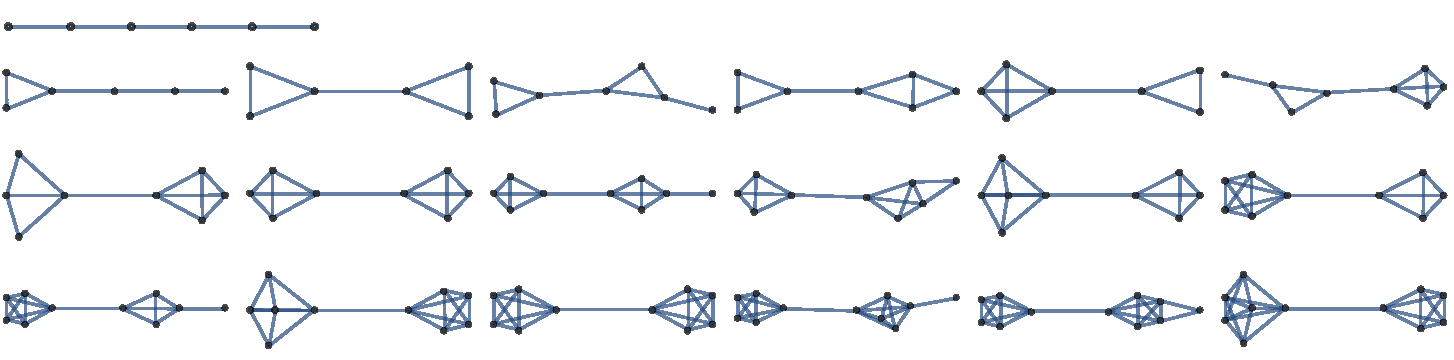
\includegraphics[width=1.0\textwidth]{MaxRatio.pdf}
\caption{\label{MaxRatio:all}In this sequence of graphs the goal was to maximise $\lambda_{2}/\lambda_{1}$. The graphs are two complete graphs joined by one edge. The parent graph is a path graph with six vertices. Not all graphs in the sequence have been plotted.}
\end{figure}

\begin{figure}
\centering
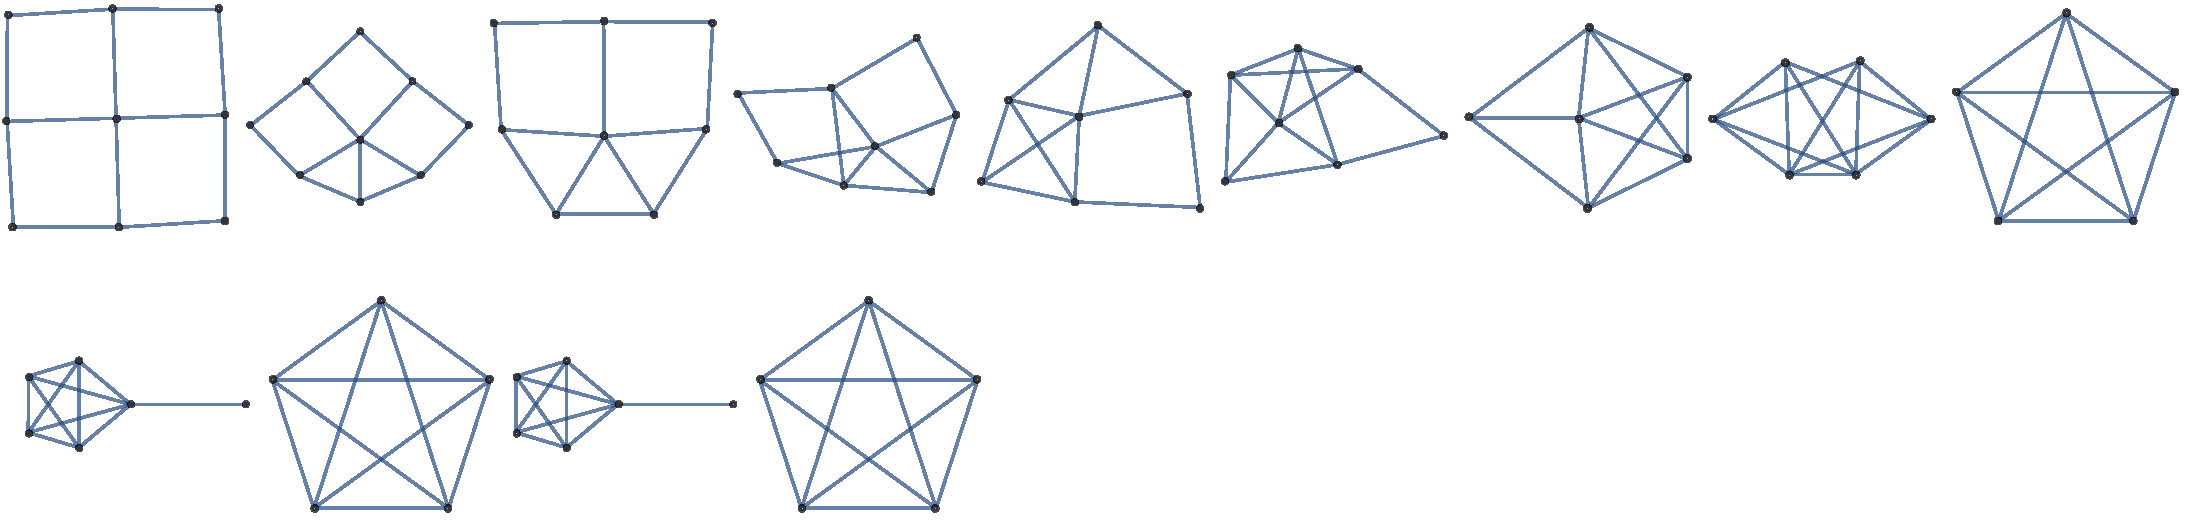
\includegraphics[width=1.0\textwidth]{GridToComplete.pdf}
\caption{\label{GridToComplete:all}In this sequence of graphs we added and then deleted an edge alternatingly, starting with a grid graph. The goal was to maximise the spectral gap, $\lambda_{1}$. The grid graph transforms to a complete graph after eight steps. The sequence then becomes cyclical, alternating between the complete graph and the complete graph with an added edge.}
\end{figure}

\begin{figure}
\centering
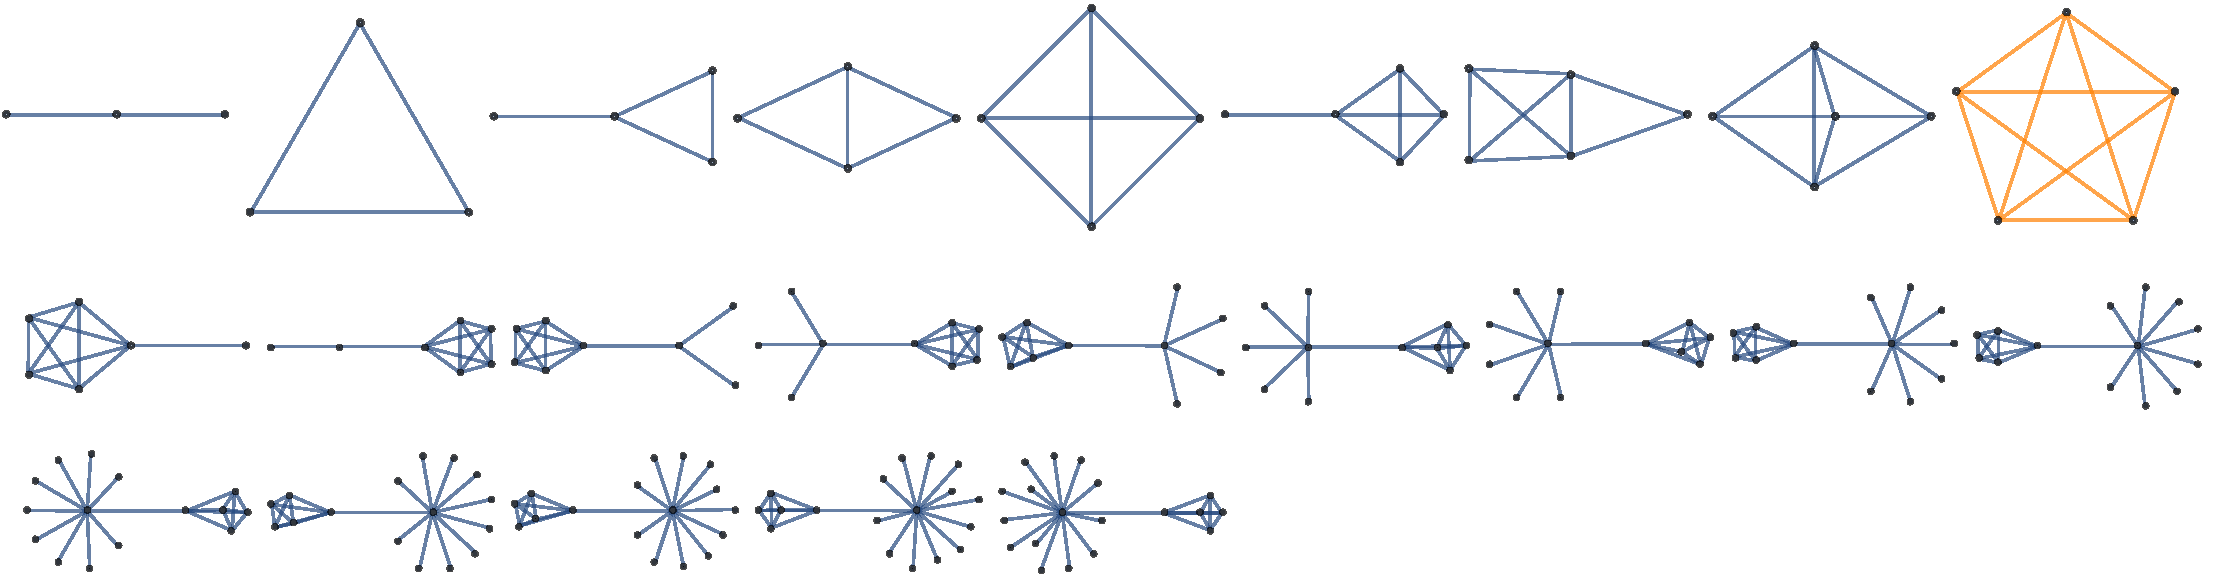
\includegraphics[width=1.0\textwidth]{Program.pdf}
\caption{\label{Program:all}In this sequence of graphs we used a program. The first goal was to increase $\lambda_{1}$ until $\lambda_{1}\geq 5\pi$ by adding an edge. This resulted in a complete graph, yellow in the figure. The goal was then changed to have a spectrum close to $(0, 5\pi,15\pi)$ by adding a vertex and an edge. The growth then proceeded as in the figure.}
\end{figure}

\section{Conclusion and outlook}
We have found that studying the growth of graphs greatly helps our intuition about their spectral properties. One immediately learns that the eigenvalues of the graphs tend to increase with increasing complexity of the graphs. In fact the graph with the smallest $\lambda_1$ is the path graph \cite{nicaise1987spectre}, where $\lambda_1=\pi^2$, which most often is our starting graph. 

We also find that the growth of graphs can help to find patterns that can be made into conjectures and one example was given above, involving the first two non-trivial eigenvalues. Not much is known about the relation between graphs and more than one non-trivial eigenvalue. 
Future work likely will involve finding more conjectures, and possibly also proving them. The fact that our program sometimes can give all solutions in an analytical form is very helpful for such research. Concerning growth of graphs there is a huge number of questions to be answered. Is it for instance possible to have something analogous to phase transitions in the graphs? That is, can a small change in the goal completely change the topology of the graph?

We have released the program that calculates spectra of graphs as open-source under Gnu General Public License \cite{Pistol2016}. The graph growth program is not released yet, since it is not very userfriendly at this stage. 
 
\newpage
\bibliographystyle{unsrt}
\bibliography{bibliography.bib}
\end{document}